% !TEX root = ../../main.tex


\section{Implementation}\label{sec:vigra_graph_lib_impl}

\todo{Impl is not a good word here}

The most important concept for graph based image processing
is the \emph{region adjacency graph} (RAG) (see \cref{fig:make_rag}).

A RAG is extracted from a labeled \emph{base graph}.
In the first step of graph based image processing, the base 
graph is usually a grid graph, and the labeling is a label image
as in \cref{fig:make_rag} .
To encode a RAG we need a undirected graph, 
and a mapping from the base graphs edges and nodes to the RAG 
needs to be stored.

The implementation of grid graphs is explained in \cref{sec:graphs_grid_graph}, 
a basic undirected graphs implementation will be discussed in \cref{sec:graphs_adjacency_list_graph}.
The implementation details of the \emph{region adjacency graph} concept will 
be given in  \cref{sec:graphs_rag}.

For hierarchical clustering we provide a specialized graph, named \emph{merge graph}.


To implemented structured clustering algorithms (see \cref{sec:rw_hc}) we
need a graph which supports the contraction of edges.
Also a mechanism to merge node and edge features is needed.
Within \cref{sec:graphs_merge_graph} we propose  a very flexible graph 
called \emph{merge graph adaptor} which fulfills these requirements.


A generic set of algorithms which work on any graph
implemented within the VIGRA graph api is presented 
in \cref{sec:graph_graph_algorithms}.

While the core implementation of any algorithm is in C++
VIGRA provides python binding to make almost
any algorithm available in Python.
To provide a generic Python interface for any proposed
graph, we need to introduce a few concepts 
to make the python wrapped graph API very \emph{Pythonic}


%$\surd \bullet$


\begin{table}
\begin{tiny}
\begin{tabular}{|l|p{1.5cm}|p{0.5cm}|p{0.5cm}|p{0.6cm}|p{0.6cm}|p{0.6cm}|p{0.8cm}|p{0.8cm}|l|l|l|}
    \hline 
    Class & purpose & 
        add nodes & add edges & contract edges & node ids & edge ids & 
        node descriptor & edge descriptors &
        node map & edge map  &
        header
    \\ \hline
    %
    2D-GridGraph & implicit graph for 2D images & 
        x & x & x & dense & sparse & 
        $\colvec{x\\y}$ &  $\colvec{x\\y\\e}$ & 
        2D-Array & 3D-Array   &
        \detokenize{multi_gridgraph.hxx}
    \\ \hline
    %
    3D-GridGraph & implicit graph for 3D volumes & 
        x & x & x & dense & sparse & 
        $\colvec{x\\y\\z}$ &  $\colvec{x\\y\\z\\e}$ & 
        3D-Array & 4D-Array   &
        \miniscule{\detokenize{multi_gridgraph.hxx}}
    \\ \hline
    %
    4D-GridGraph & implicit graph for 3D volumes $+$ time & 
        x & x & x & dense & sparse & 
        $\colvec{x\\y\\z\\t}$ &  $\colvec{x\\y\\z\\t\\e}$ & 
        4D-Array & 5D-Array   &
        \detokenize{multi_gridgraph.hxx}
    \\ \hline
    %
    AdjacencyListGraph & multi purpose graph & 
       $\bullet$  & $\bullet$ & x & maybe dense & dense & 
       $\colvec{n}$ , same as node id &  $\colvec{e}$  , same as edge id & 
       1D-Array & 1D-Array   &
       \detokenize{adjacency_list_graph.hxx}
    \\ \hline
    %
    MergeGraphAdpator & edge contraction with feature merging callback & 
       x & x & $\bullet$& sparse & sparse & 
       $\colvec{n}$ , same as node id &  $\colvec{e}$ , same as edge id & 
       1D-Array & 1D-Array   &
       \detokenize{merge_graph_adaptor.hxx}
    \\ \hline
\end{tabular}
\end{tiny}
\end{table}
\subsection{Graphs}

\subsubsection{Grid Graph} \label{sec:graphs_grid_graph}

The grid graph implemented in VIGRA is N-dimensional.
The dimension can be selected with templates, and therefore with zero
overhead.

Due to the regular structure of a grid graph, it is possible to compute the edges of a given 
node and vice versa on the fly, instead of storing these relations explicitly.
Therefore a grid graph can be implemented with almost zero memory overhead.

\paragraph{Node Descriptor/Id :}
The node descriptor of a grid graph is implemented as a
$N$-dimensional coordinate of the pixel which corresponds to
that particular node. The id of a node is the scan order index
of the corresponding pixel.
As a consequence, node id's of a grid graph are continuous.
\paragraph{Edge Descriptor/Id :}
To edge descriptors are implemented as $N+1$-dimensional coordinate.
The first $N$ axis correspond to the node which ``owns'' this edge.
The last axis enumerates the edge w.r.t. the node.

In a grid graph, all nodes have the same degree, except for nodes
at the border of the image.
This breaks somehow the regularity of grid graphs.
To still have very regular structure, edge ids
are enumerated, as if the graph would be perfectly
regular. Therefore we enumerate some missing edges
at the border and get non-continuous edge ids.
\Cref{fig:grid_graph_ids} illustrates this enumeration.



\begin{figure}[H]
\centering
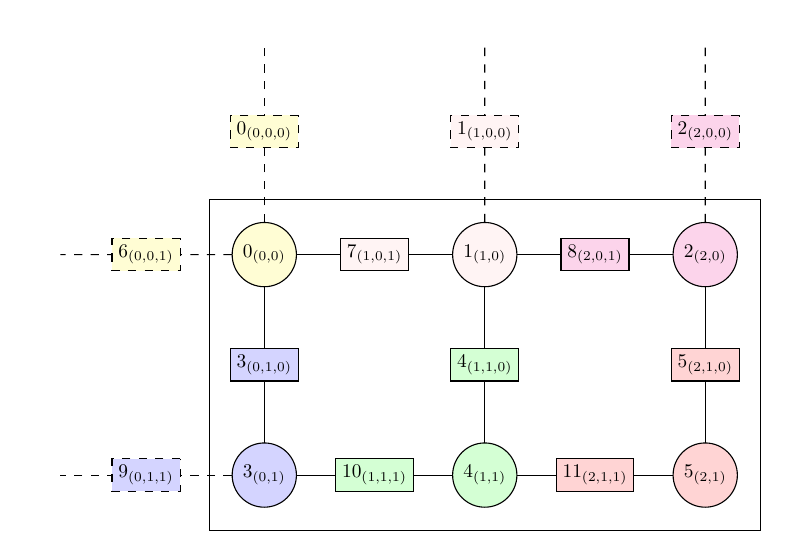
\begin{tikzpicture}[scale=0.7,transform shape]
  % virtual nodes
  \draw (-2*2,0) node (naa) {$\quad$};
  \draw (-2*2,2*2) node (nbb) {$\quad$};
  \draw (0,4*2) node (na) {$\quad$};
  \draw (2*2,4*2) node (nb) {$\quad$};
  \draw (4*2,4*2) node (nc) {$\quad$};
  % real nodes
  \draw (0,0) node[draw,circle,fill=blue!17] (n3) {$3_{(0,1)}$};
  \draw (2*2,0) node[draw,circle,fill=green!17] (n4) {$4_{(1,1)}$};
  \draw (4*2,0) node[draw,circle,fill=red!17] (n5) {$5_{(2,1)}$};
  \draw (0,2*2) node[draw,circle,fill=yellow!17] (n0) {$0_{(0,0)}$};
  \draw (2*2,2*2) node[draw,circle,fill=pink!17] (n1) {$1_{(1,0)}$};
  \draw (4*2,2*2) node[draw,circle,fill=magenta!17] (n2) {$2_{(2,0)}$};
  %
  % real edges
  \path[every node/.style={auto=false}]
    (n0) edge node[draw,rectangle,fill=pink!17] {$7_{(1,0,1)}$} (n1) 
    (n1) edge node[draw,rectangle,fill=magenta!17] {$8_{(2,0,1)}$} (n2) 
    (n3) edge node[draw,rectangle,fill=green!17] {$10_{(1,1,1)}$} (n4) 
    (n4) edge node[draw,rectangle,fill=red!17] {$11_{(2,1,1)}$} (n5);
 \path[every node/.style={auto=false}]
    (n0) edge node[draw,rectangle,fill=blue!17] {$3_{(0,1,0)}$} (n3) 
    (n1) edge node[draw,rectangle,fill=green!17] {$4_{(1,1,0)}$} (n4) 
    (n2) edge node[draw,rectangle,fill=red!17] {$5_{(2,1,0)}$} (n5) ;
  %
  %virtual edges x
  \path[every node/.style={auto=false}]
    (n0) edge[dashed] node[draw,rectangle,fill=yellow!17] {$0_{(0,0,0)}$} (na) 
    (n1) edge[dashed] node[draw,rectangle,fill=pink!17] {$1_{(1,0,0)}$} (nb) 
    (n2) edge[dashed] node[draw,rectangle,fill=magenta!17] {$2_{(2,0,0)}$} (nc) ;
  \path[every node/.style={auto=false}]
    (n0) edge[dashed] node[draw,rectangle,fill=yellow!17] {$6_{(0,0,1)}$} (nbb) 
    (n3) edge[dashed] node[draw,rectangle,fill=blue!17] {$9_{(0,1,1)}$} (naa) ;
   %
   \draw (-1.0,5.0) --  (9,5.0) -- (9,-1.0) -- (-1.0,-1.0) -- cycle;
\end{tikzpicture}
\caption[Grid Graph Ids]{ \label{fig:grid_graph_ids}
    Ids and descriptors for a 2D Grid graph with 4-neighborhood on a $3x2$ grid.
    The node ids are continuous from $0$ to $5$ and the descriptors
    are showed as subscripts of the ids.
    Node descriptors are 2D pixel coordinates.
    To get the edge ids, we enumerate the edge, but we ignore the fact that nodes at the
    left and upper border do
    not have an upper and left edge.
    To illustrate this, these ``virtual'' edges are shown dotted.
    The id's of the edges correspond to the enumeration.
    As a consequence edge ids are non continuous.    
    In this examples, 
    the set of valid edge ids is $\{ 3,4,5,7,8,10,11 \}$.
    Edge descriptors are 3D coordinates, where the first two
    coordinate correspond to the node which owns this edge.
    The third coordinate is the edge number w.r.t. the node.
    The two edges and the node which ``owns'' them are
    shown in the same unique color.

}
\end{figure}

\paragraph{Node Map :} An regular N-dimensional image can
be used as node map, and since node descriptors are plain
coordinates, they can be used to access data at a
particular pixel.
This means, no node map needs to be allocated for a given
image, since the image itself can be used as a node map.
The default node map is derived from \lstinline{vigra::MultiArray<DIM,T>}.

\paragraph{Edge Map :} An N+1-dimensional image is
used as edge map.
This image has the same as a node map, but an extra
dimension for the edges.
The first $N$ axis in the edge descriptor are 
used to determine which pixel ``owns'' the edge,
while the last axis select the w.r.t. the node.
The default edge map is derived from \lstinline{vigra::MultiArray<DIM,Multiband<T> >}.

\paragraph{Usage :}

\subsubsection{Adjacency List Graph} \label{sec:graphs_adjacency_list_graph}

\paragraph{Node Descriptor/Id :}
The node descriptor is implemented as a simple class
holding a single integer which is the id 
of the node.
The user can explicitly choose the id of
an node. As a consequence, node id's can 
be sparse and continuous.

\paragraph{Edge Descriptor/Id :}
The edge descriptors are implemented exactly like
node descriptors, but users cannot give
edges explicit id's.
Therefore edge id's are dense, unless
edges are removed from the graph \footnote{Removing edges from the graph is
not yet implemented}.

\paragraph{Node Map, EdgeMap:} 
The node and edge maps are derived from \lstinline{vigra::MultiArray<1,T>}.
Their size is to \lstinline{maxNodeId()+1} and  \lstinline{maxEdgeId()+1}.
The id and the descriptors can be used to index node and edge maps.


\paragraph{Usage :}
    \begin{lstlisting}[language=c++]
    typedef vigra::AdjacencyListGraph Graph;
    Graph g;

    // add nodes 
    // - automatic id
    // - explicit id
    Graph::Node n0 = g.addNode() 
    Graph::Node n3 = g.addNode(3)

    // add edges from existing nodes
    // and new nodes
    // no parallel edges 
    Graph::Edge e0 = g.addEdge(n0,n1)
    Graph::Edge e1 = g.addEdge(2,3)
    Graph::Edge e2 = g.addEdge(2,3)
    assert(e1==e2)  
    \end{lstlisting}

    \begin{lstlisting}[language=Python]
    g=vigra.graphs.listGraph();
    # add nodes 
    # - automatic id
    # - explicit id
    n0 = g.addNode() 
    n3 = g.addNode(3)

    # add edges from existing nodes
    # and new nodes
    # no parallel edges 
    e0 = g.addEdge(n0,n1)
    e1 = g.addEdge(2,3)
    e2 = g.addEdge(2,3)
    assert e1==e2  
    \end{lstlisting}
\subsubsection{Region Adjacency Graph} \label{sec:graphs_rag}







To map edges and nodes from the base graph


\subsubsection{Merge Graph} \label{sec:graphs_merge_graph}

To implemented structured clustering algorithms (see \cref{sec:rw_hc} ) 
A graph which supports edge contraction and feature merging is needed.
Some graphs within the LEMON library support 
edge contraction, but this is not part of LEMON undirected graph concept \footnote{
Edge contraction cannot be a part of LEMON undirected graph concept,since some graphs
are not mutable.}.

\begin{figure}[H]
    \centering
    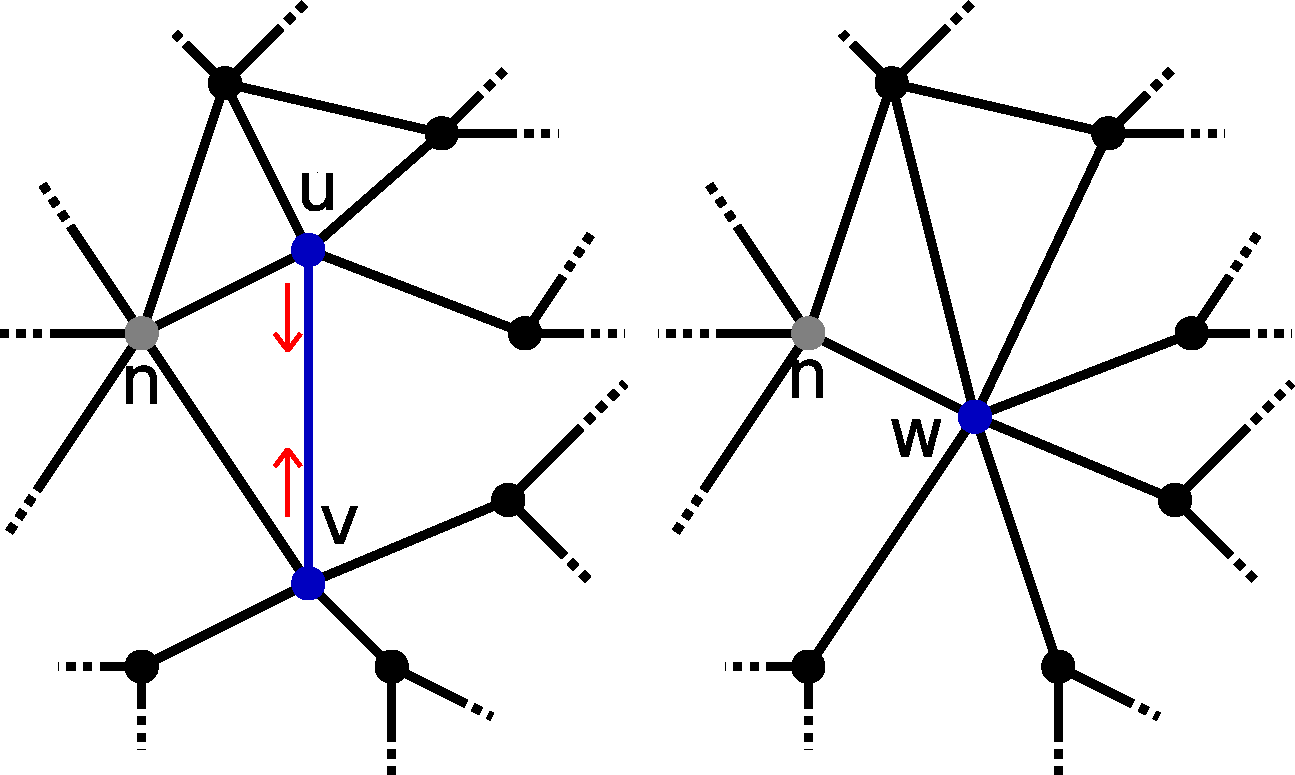
\includegraphics[width=0.35\textwidth]{fig/contraction.pdf}

    \addtocontents{lof}{%
        \vspace{1cm}
        \protect\centerline{%
            \protect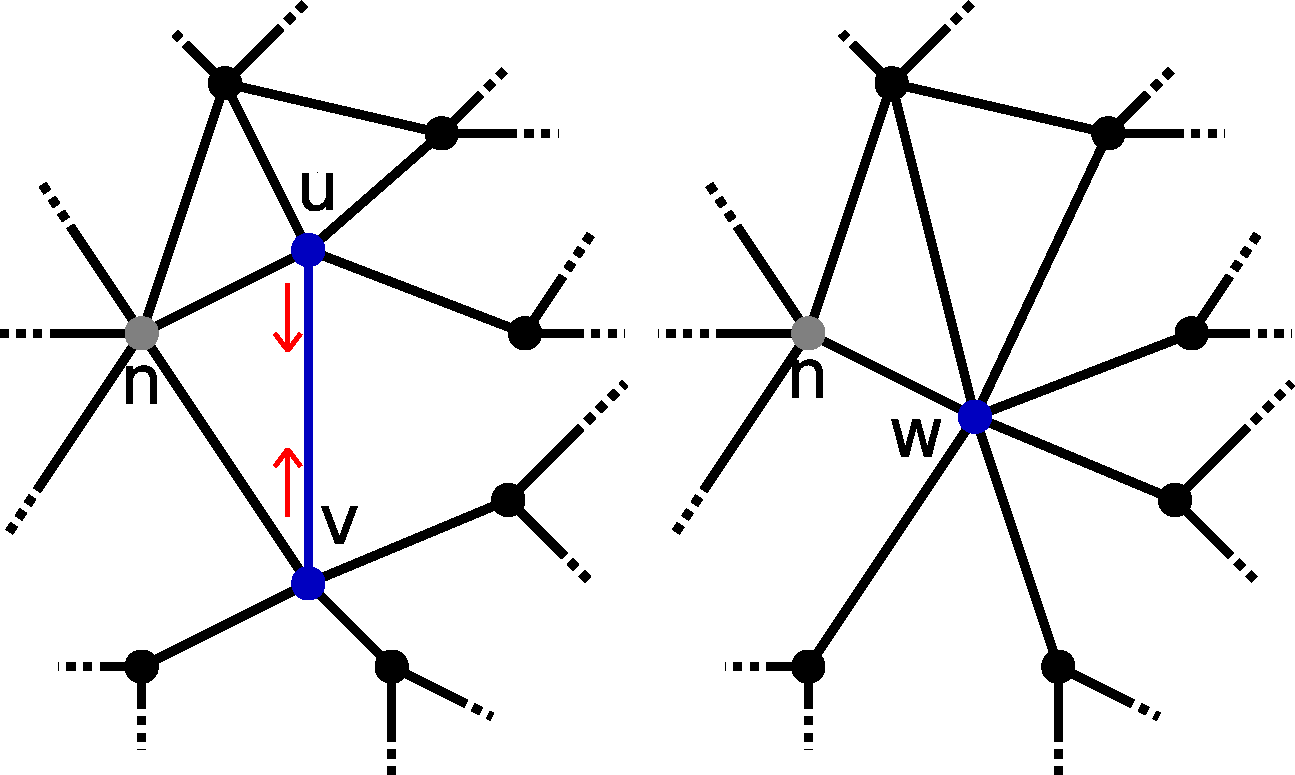
\includegraphics[width=\lofthumbsize,height=\lofthumbsize,keepaspectratio=true]{fig/contraction.pdf} 
        } 

    }%
    \caption[Schematic edge contraction]{ Schematic edge contraction: Node $u$ and $v$ is merged into node $w$.
        Note the gray node $n$ which is connected to $u$ and $v$.
        After the contraction, edges $\{ n,u\}$ and $\{ n,v\}$ are also merged into 
        a single edge $\{ n, w\}$.
        The picture has been taken from \citep{wiki_edge_contraction} and has been modified slightly.
    }
    \label{fig:figlabel}
\end{figure}


Furthermore LEMON does not define any concept for feature merging, which
is crucial for image processing application \citep{arbelaez_2006_cvpr}.
As a consequence, we define a new concept / API for 
edge contraction and feature merging within the philosophy of LEMON.

We implemented the \emph{merge graph} as an LEMON  \href{http://lemon.cs.elte.hu/pub/doc/latest/a00592.html}{graph adaptor}
\footnote{ LEMON Graph Adaptor: \url{http://lemon.cs.elte.hu/pub/doc/latest/a00592.html} }.
A graph adaptor is aways a viewing to a base graph and cannot exist without one.
A subgraph adaptor can used to get view to a subgraph w.r.t. the base graph, without
the need to reallocate the complete subgraph.
In a similar manner, we implement a \emph{merge graph adaptor}.

Each node and edge in the merge graph adaptor corresponds to a connected component of 
edge and nodes in the base graph.
Two union find data structure (UFD), and edge and node ufd encode these connected components.

Feature merging is done via \emph{callbacks} which can be registered to the merge graph adaptor.
The \emph{callback API} is explained in detail below. 


\begin{figure}[H]
\begin{center}
    \begin{tikzpicture}[scale=0.65,transform shape]
        \umlclass[template=Graph]{MergeGraphAdpator}
        {
            - edgeUfd               : IterablePartiton          \\
            - nodeUfd               : IterablePartiton          \\ 
            - nodesAdjacency        : AdjacencySetVector        \\
            - baseGraph             : Graph                     \\
            - mergeNodeCallBacks    : MergeNodeCallBackVector   \\
            - mergeEdgeCallBacks    : MergeEdgeCallBackVector   \\
            - eraseEdgeCallBacks    : EraseEdgeCallBackVector   
        }
        {
            // LEMON API for undirected graphs                  \\
                $\ldots$                                        \\
            // register callbacks                               \\ 
            + registerMergeNodeCallBack(f : MergeNodeCallBack)  \\
            + registerMergeEdgeCallBack(f : MergeEdgeCallBack)  \\
            + registerEraseEdgeCallBack(f : EraseEdgeCallBack)  \\
            // modify graph                                     \\
            + contractEdge(edge : Edge)     : Node              \\
            // find representatives                             \\
            + reprNode(node : Graph::Node)  : Node              \\
            + reprEdge(edge : Graph::Node)  : Edge              \\ 
            // get base graph                                   \\
            + graph()                       : Graph             \\
        } 
    \end{tikzpicture}
\end{center}\caption[Merge Graph Adaptor Class Diagram]{ \label{fig:cls_mga}
    Merge Graph Adaptor Class Diagram.
    Only member functions which are not part of the LEMON
    undirected graph concept are listed. 
    See \cref{fig:uml_lemon_graph_concepts} for all missing 
    members.
}
\end{figure}



\paragraph{Node Descriptor/Id :}
The node descriptor is implemented as a simple class
holding a single integer which is the id 
of the node.
Each node in the merge graph encodes a connected
component of nodes in the base graph.
If no edge has been contracted, the node ids
of the merge graph are identical with the ids 
of the base graph.
The contraction of a single edge will invalidate
one node id, since two nodes are merged into a single 
node.
The connected component membership of base graph
nodes is stored in a union find data structure 
and can be accessed via \lstinline{MergeGraph::reprNode(const BaseGraphNode & baseGraphNode)}.


\paragraph{Edge Descriptor/Id :}
Edge descriptors are implemented as node descriptors.
The contraction of a single edge will invalidate
at least one edge id, since the contracted edge is removed
from the graph.
But contracting a single edge can lead to an
unbounded number of parallel edges / multi edges.
Multiple edges between a pair of nodes will be merged
into single edges.
The connected component membership of base graph
edges is stored in a union find data structure 
and can be accessed via \lstinline{MergeGraph::reprEdge(const BaseGraphEdge & baseGraphEdge)}.
This is only defined if $u,v$-nodes of this edge are in different connected components.



\paragraph{Node Map, EdgeMap :} 
The node and edge maps are derived from \lstinline{vigra::MultiArray<1,T>}.
Their size is to \lstinline{maxNodeId()+1} and  \lstinline{maxEdgeId()+1}.
The id and the descriptors can be used to index node and edge maps.
The implementation is exactly the same as for the AdjacencyListGraph \Cref{sec:graphs_adjacency_list_graph}.
The default implementation of node and edge maps does not perform 
any feature merging since the merging strategy depends on the
features and the application itself.
To perform feature merging the merge graph uses a callback API which is explained below.


\paragraph{Callback API :}

To merge features the merge graph uses three different callbacks types.
Any of these callbacks is implemented within boosts API for callbacks \citep{ boost_function}
\footnote{
Currently we use the boost implementation for callbacks, but 
in the future we might use a faster implementation with the same API  \citep{code_project_function}.
}.


\begin{compactitem}
\item Merge node callback :
    A contraction of an edge merges the two nodes of the edge
    into a single node.
    To merge node features a callbacks with the following signature 
    can be registered to the merge graphs merge node callback vector.
    \\
    \lstinline[language=c++]{void mergeNodeSignature(const Node & anchorNode,const Node & deadNode);}
    \\
    The first argument is the anchor node, therefore the id and descriptor of
    \lstinline{anchorNode} are still  valid after the contraction, while
    the  id and descriptor of \lstinline{deadNode} become invalid.


\item Merge node callback :
    A single edge contraction can lead to multiple parallel edges
    which will be merged into single edges.
    To merge features attached to edges, a callback vector
    similar to the node callback vectors exists.
    The signature is the same as for node callbacks, only with 
    edge descriptors.
    \\
    \lstinline[language=c++]{void mergeEdgeSignature(const Edge & anchorEdge,const Edge & deadEdge);}
    \\
    Again, the first argument is the anchor, and ids and descriptors stay valid.
    The id and descriptor of the second argument become invalid after the merge.

\item Erase edge callback :
    The edge which is contracted is removed from the graph.
    This callback can be used to inform data structures 
    that this edge has been removed.
    \\
    \lstinline[language=c++]{void eraseEdgeSignature(const Edge & edge);}
    \\
    Furthermore this callback is called at the very and of each
    edge contraction. Therefore this callback can be used
    to indicate that all callbacks have been called and
    the contraction is finished.

\end{compactitem}





   





\subsection{Graph Algorithms} \label{sec:graph_graph_algorithms}

    \subsubsection{Multicut}

    \subsubsection{Hierarchical Clustering}

    \begin{center}
    \begin{tikzpicture}[scale=0.7,transform shape]
    \begin{umlpackage}{Hierarchical Clustering Class Design / Class Hierarchy}
        \umlclass[x=-3,template=Graph]{MergeGraphAdpator}
        {
            \\// union find data structures                     \\
            - edgeUfd               : IterablePartiton          \\
            - nodeUfd               : IterablePartiton          \\ 
            - nodesAdjacency        : AdjacencySetVector        \\

            \\// ref. to base graph                             \\
            - baseGraph             : Graph                     \\
            \\// callbacks                                      \\
            - mergeNodeCallBacks    : MergeNodeCallBackVector   \\
            - mergeEdgeCallBack     : MergeEdgeCallBackVector   \\
            - eraseEdgeCallBack     : EraseEdgeCallBackVector   \\
        }
        {
            \\// LEMON API for undirected graphs                \\
                $\ldots$                                        \\
            \\// register callbacks                             \\ 
            + registerMergeNodeCallBack(f : MergeNodeCallBack)  \\
            + registerMergeEdgeCallBack(f : MergeEdgeCallBack)  \\
            + registerEraseEdgeCallBack(f : EraseEdgeCallBack)  \\

            \\// modify graph                                   \\
            + contractEdge(edge : Edge)     : Node              \\

            \\// find representatives                           \\
            + reprNode(node : Graph::Node)         : Node       \\
            + reprEdge(edge : Graph::Edge)         : Edge       \\ 

            \\// get base graph                                 \\
            + graph()                       : Graph             \\
        } 


        \umlclass[x=6,y=3,template=MergeGraph]{ClusterOperatorInterface}
        {

        }
        {
            \\// contract next edge and get weight              \\
            + contractionEdge(edge : Edge)         : Edge       \\ 
            + contractionWeight(edge : Edge)       : Edge       \\
            \\// get base graph                                 \\
            + mergeGraph()                  : MergeGraph        \\
        } 


        \umlclass[x=9,y=-5,template=ClusterOperator]{HierarchicalClustering}
        {

        }
        {
            + cluster()                     : void        \\
            + reprLabels(nodeMap : NodeMap) : void        \\      
        } 

        \umldep[geometry=-|-,name=cb]{MergeGraphAdpator}{ClusterOperatorInterface}
        \umldep[geometry=-|-,name=dep2]{ClusterOperatorInterface}{HierarchicalClustering}

        \umlnote[x=3,y=-3]{cb-2}{
            ClusterOperator registers callbacks to MergeGraph
        }
        
        \umlnote[x=12,y=2]{ClusterOperatorInterface}{
            Responsible for feature merging.
            Finds next edge to contract. 
        }
        \umlnote[x=12,y=-8]{HierarchicalClustering}{
            Encodes merge tree / dendrogram. 
        }


    \end{umlpackage}
    \end{tikzpicture}
    \end{center}

    \subsubsection{Watershed Algorithms}

    \subsubsection{Smoothing Algorithms}

